\author{João Gonçalves}
\newcommand{\authorr}{Teresa Nogueira}
\newcommand{\studentID}{99995}
\newcommand{\studentIDD}{100029}
%\newcommand{\supervisorone}{Prof\textsuperscript{\underline{a}}. XXXXXX}
\newcommand{\supervisorone}{}
\newcommand{\supervisortwo}{}
\newcommand{\department}{Engenharia Eletrotécnica e de Computadores}
\newcommand{\exam}{Controlo}

\title{%
Apontamentos sobre Controlo\\
\large (Alguns tópicos \href{https://github.com/Kons-5}{\raisebox{0 em}{\large \faGithub}})}
\date{Maio 2023}

\documentclass[a4paper,12pt]{article}
\usepackage[left=25mm,top=21mm,right=25mm,bottom=21mm]{geometry}
\usepackage[flushmargin,hang,bottom,multiple]{footmisc}
\usepackage[usestackEOL]{stackengine}
\usepackage{babel}
\usepackage[T1]{fontenc}
\usepackage[utf8]{inputenc}
\usepackage{fontawesome5,textcomp}
\usepackage{xcolor}
\usepackage{fancyhdr}

\usepackage[export]{adjustbox}
\usepackage{graphicx,array,tabularx}
\usepackage{float,wrapfig}
\usepackage[font=footnotesize, labelfont=bf]{caption}
\usepackage[justification=centering]{subcaption}

\usepackage{amsmath,amsfonts,amssymb}
\usepackage{bm}
\usepackage{mathtools}
\usepackage{mathabx}
\usepackage{physics}
\usepackage{cancel}
\usepackage{empheq}

\usepackage{pgfplots}
\usepackage{msc}
\usepackage{booktabs}
\usepackage{tcolorbox}
\usepackage{etoolbox}

\usepackage{makecell}
\usepackage{listings}
\usepackage{enumitem}

\usepackage[linktoc=all]{hyperref}
\usepackage[capitalise]{cleveref}
\usepackage[nottoc,numbib]{tocbibind}
\usepackage[square,numbers,sort]{natbib}
\usepackage{breakurl}
\usepackage{placeins}
\usepackage{colortbl}
\usepackage{attrib}
\usepackage{multirow,multicol}

%\usepackage[printwatermark]{xwatermark}
\usepackage[framemethod=TikZ]{mdframed}
%\tcbuselibrary{skins,breakable}
%\usetikzlibrary{shadings,shadows}
\linespread{1}
%\setlength{\parindent}{0pt}

\hypersetup{
    colorlinks,
    linkcolor={black},
    citecolor={blue!50!black},
    urlcolor={blue!50!black}
}

\setlength{\abovedisplayskip}{3pt}
\setlength{\belowdisplayskip}{3pt}
\setlength{\fboxsep}{1.25\fboxsep}

\newcommand*\widefbox[1]{\fbox{\hspace{2em}#1\hspace{2em}}}

\let\zzzfootnotesize\footnotesize
\def\newfootnotesize{%
\zzzfootnotesize
\abovedisplayskip=0pt
\belowdisplayskip=\abovedisplayskip
\abovedisplayshortskip=\abovedisplayskip
\belowdisplayshortskip=\abovedisplayskip
}
\renewcommand\footnotesize{\protect\newfootnotesize}

\mdfsetup{%
    linewidth=2pt
}
%//==============================--@--==============================//%
%                         -> error messages <-                        %
\usepackage{pifont}

\newenvironment{warning}
  {\par\begin{mdframed}[linewidth=1.5pt,linecolor=red]%
    \begin{list}{}{\leftmargin=0.9cm
                   \labelwidth=\leftmargin}\item[\raisebox{-0.4 em}{\Large\ding{43}}]}
  {\end{list}\end{mdframed}\par}

%//==============================--@--==============================//%
%                   -> reduzir espaço entre itens <-                  %
\usepackage{enumitem}
%\setlist[itemize]{nosep}
%\setlist[enumerate]{nosep}
\setlist[itemize]{itemsep=0.0125em}
\setlist[enumerate]{itemsep=0.0125em}
%//==============================METH-==============================//%
\newcounter{theo}[section]\setcounter{theo}{0}
\renewcommand{\thetheo}{\arabic{theo}}

%\definecolor{tempcolor}{RGB}{113, 110, 97}
\definecolor{tempcolor}{RGB}{0, 0, 0}
\newenvironment{theo}[2][]{%
    \refstepcounter{theo}
    \ifstrempty{#1}%
    % if condition (without title)
    {\mdfsetup{%
        frametitle={%
            \tikz[baseline=(current bounding box.east),outer sep=0pt]
            \node[anchor=east,rectangle,fill=blue!20]
            {\strut Teorema~\thetheo};}
        }%
    % else condition (with title)
    }{\mdfsetup{%
        frametitle={%
            \tikz[baseline=(current bounding box.east),outer sep=0pt]
            \node[anchor=east,rectangle,fill=white]
            {\strut #1};}%
        }%
    }%
    % Both conditions
    \mdfsetup{%
        innertopmargin=0pt,linecolor=tempcolor,%
        linewidth=2pt,topline=true,%
        frametitleaboveskip=1.25\dimexpr-\ht\strutbox\relax%
    }
 
\begin{mdframed}[]\relax\vspace{-0.5em}}{%
\end{mdframed}}

\def\delequal{\mathrel{\ensurestackMath{\stackon[1pt]{=}{\scriptstyle\Delta}}}}

\let\originalleft\left
\let\originalright\right
\renewcommand{\left}{\mathopen{}\mathclose\bgroup\originalleft}
\renewcommand{\right}{\aftergroup\egroup\originalright}
%------------------------------------ MAGIC--------------------------------------
\def\UrlBreaks{\do\/\do-}
\expandafter\def\expandafter\UrlBreaks\expandafter{\UrlBreaks\do\a%
\do\b\do\c\do\d\do\e\do\f\do\g\do\h\do\i\do\j\do\k\do\l\do\m\do\n%
\do\o\do\p\do\q\do\r\do\s\do\t\do\u\do\v\do\w\do\x\do\y\do\z\do\&}

\newcolumntype{C}[1]{>{\centering\let\newline\\\arraybackslash\hspace{0pt}}m{#1}}
\newcolumntype{L}[1]{>{\raggedright\let\newline\\\arraybackslash\hspace{0pt}}m{#1}}
%----------------------------------TITLE PAGE -----------------------------------
\makeatletter
\def\maketitle{
  \begin{center}\leavevmode
        \normalfont
        
\includegraphics[width=0.35\columnwidth]{img/title-page/IST.pdf}
        \vskip 0.05cm   
        \textsc{\large \department}\\
        \vskip 0.5cm
        \rule{0.95\linewidth}{0.2 mm} %\\
        {\large \exam}\\[0.5 cm]
        {\huge \bfseries \@title \par} 
        \vspace{1em}
        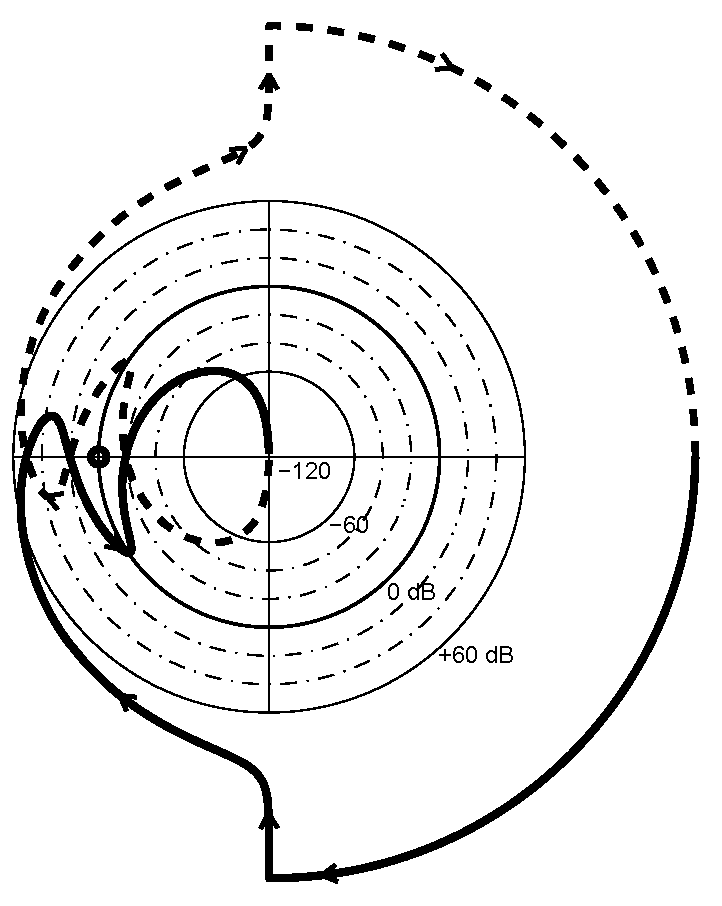
\includegraphics[scale=0.4]{img/title-page/000.png}
        %\vspace{0.5cm}
        \rule{0.95\linewidth}{0.2 mm} \\[0.75 cm]
        %\fontsize{9pt}{11pt}\selectfont
        \begin{minipage}[t]{1\textwidth}
	   \begin{flushleft} \large
                \emph{Autores:}\\
			\normalsize \textbf{\@author} : \studentID\\
                \fontsize{9pt}{11pt}\selectfont $\hookrightarrow$ jrazevedogoncalves@tecnico.ulisboa.pt \\
                \normalsize \textbf{\authorr} : \studentIDD\\
                \scriptsize $\hookrightarrow$ maria.teresa.ramos.nogueira@tecnico.ulisboa.pt
		\end{flushleft}
	\end{minipage}

    \vfill
	{\Large \@date\par}
   \end{center}
   %\vfill
   %\null
   \cleardoublepage
  }
\makeatother
%-------------------------------- ENDTITLE PAGE ----------------------------------
%---> Header <---
%\fancyhf{}
\renewcommand{\headrulewidth}{1pt}% Header rule width
\renewcommand{\footrulewidth}{0pt}% No footer rule
\setlength\headheight{26pt} 
\fancyhead[L]{\raisebox{0.1\height}[0pt][0pt]{\textit{Controlo}}}
\fancyhead[R]{\raisebox{0.1\height}[0pt][0pt]{2022/2023}}
%%%%%%%%%%%%%%%%%

\pgfplotsset{compat=1.18}
\setcounter{tocdepth}{3}
%\setcounter{secnumdepth}{4}
\setcounter{secnumdepth}{-2}

\renewcommand{\figurename}{Fig.}
\renewcommand{\tablename}{Tab.}
\renewcommand{\contentsname}{Índice}
\settocbibname{\raisebox{0em}{Referências}}
\setlength{\bibsep}{0.15em}%reduzir espaço entre refs.

%\renewcommand{\bibpreamble}{\vspace{-8em}}
\usepackage[titles]{tocloft}
\setlength{\cftbeforesecskip}{0.35em}

%\usepackage{pdfpages}
% \newwatermark[page=15,fontfamily=bch,color=red!50,angle=45,scale=3.5,xpos=-10,ypos=10]{TO BE ADDED}


\begin{document}
    \sloppy
    %% title page
    \pagenumbering{gobble}
    \maketitle
    %% toc
    \tableofcontents
    \setcounter{tocdepth}{4}
    %% body
    \newpage
    \pagestyle{fancy}
    \pagenumbering{arabic}

    \clearpage
    \section{Modelação e Linearização}\label{sec:Modelacao_e_Linearizacao}%
        %//==============================--@--==============================//%
\subsection[2.1 Linearização de Sistemas Não Lineares]{\hspace*{0.075 em}\raisebox{0.2 em}{$\pmb{\drsh}$} Linearização de Sistemas Não Lineares}
\label{sec:linearisation}

\noindent A aproximação linear de uma função é o \underline{polinómio de Taylor de primeira ordem} em torno do ponto de interesse. Em sistemas dinâmicos, é um método que permite (possivelmente) aferir a estabilidade local de pontos de equilíbrio de sistemas não lineares.

{
\mdfsetup{linewidth=2pt}

\begin{mdframed}
    \noindent Seja $\pmb{\dot{x}} = f(\pmb{x})$, não linear. A equação geral para a linearização de uma função multivariável $f(\pmb{x})$ num ponto $\pmb{p}$ é:
    \vspace{-0.5em}
    $$
        f(\pmb{x}) \approx f(\pmb{p}) + \left.D f\right|_{\pmb{p}} \cdot (\pmb{x} - \pmb{p})
    $$
    
    \noindent onde $\pmb{x}$ é o vetor de variáveis e $\pmb{p}$ o ponto de interesse para a linearização.
\end{mdframed}
}

\begin{quote}
    \noindent ``A good place to start analyzing the nonlinear system 
    $$
        \pmb{\dot{x}} = f(\pmb{x}) 
    $$
    is to determine its \underline{equilibrium points} and describe its behavior near [this points]. (...) the local behavior of the nonlinear system near a hyperbolic equilibrium point $\pmb{p}$ is qualitatively determined by the behavior of the linear system
    $$
        \pmb{\dot{x}} = \pmb{A}\,\pmb{x},
    $$
    with the matrix $\pmb{A} = Df(\pmb{p})$, near the origin. 
    
    The linear function $\pmb{A}\, \pmb{x} = Df(\pmb{p})\, \pmb{x}$ is called the \textit{linear part} of $f$ at $\pmb{p}$.''\cite{Perko2013}
\end{quote}

%//==============================--@--==============================//%
        \renewcommand*{\thefootnote}{\fnsymbol{footnote}}
\def\equalfootnote{\mathrel{\ensurestackMath{\stackon[0.5pt]{=}{\footnotemark[2]}}}}

\makeatletter
\newcommand{\smallbullet}{} % for safety
\DeclareRobustCommand\smallbullet{%
  \mathord{\mathpalette\smallbullet@{0.75}}%
}
\newcommand{\smallbullet@}[2]{%
  \vcenter{\hbox{\scalebox{#2}{$\m@th#1\bullet$}}}%
}
\makeatother
%//==============================--@--==============================//%
\subsection[2.2 Modelação de Sistemas Físicos]{\hspace*{0.075 em}\raisebox{0.2 em}{$\pmb{\drsh}$} Modelação de Sistemas Físicos}
\label{sec:mechanics}
%//==============================--@--==============================//%
\subsubsection[2.2.1 Sistemas Mecânicos de Translação]{$\pmb{\rightarrow}$ Sistemas Mecânicos de Translação}
\label{sec:mechanics-translation}

\begin{quote}
    ``The cornerstone for obtaining a mathematical model, or the dynamic equations, for any mechanical system is Newton's law
    $$
        \boxed{F = \frac{dp}{dt} = \frac{d}{dt} (m v) \equalfootnote ma}
    $$
    \noindent where:
    \begin{itemize}[leftmargin=*,label=${\smallbullet}$]
        \item $F$ = the vector sum of all forces applied to each body in a system, newtons (N),
        \item $p$ = linear momentum/translational momentum (kg ms$^{-1}$),
        \item $v$ = velocity (ms$^{-1}$), the directional speed of an object in motion as an indication of its rate of change in position as observed from a particular frame of reference,
        \item $a$ = the vector acceleration of each body with respect to an inertial reference frame (that is, one that is neither accelerating nor rotating with respect to the stars); often called inertial acceleration, ms$^{-2}$,
        \item $m$ = mass of the body, kg.''\cite{FranklinPowell2015}
    \end{itemize}
\end{quote}

\footnotetext[2]{Para uma massa invariante no tempo, ou aproximadamente constante.}
\renewcommand*{\thefootnote}{\arabic{footnote}}

\phantomsection\addcontentsline{toc}{subsubsection}{3.1.1 Relações fundamentais baseadas em princípios físicos}
\renewcommand*{\thefootnote}{\fnsymbol{footnote}}
\begin{theo}[\underline{Molas Elásticas}]{def:Molas Elásticas}\label{def:MolasElásticas}
Quando uma mola é comprimida ou esticada, reage com uma força que se opõe à compressão (ou à extensão). Força desta que, para molas lineares, é dada por:
$$
    f = -kx
$$
Onde $k$ é a constante de Hooke [N/m].
\end{theo}

\begin{theo}[\underline{Atrito Viscoso}]{def:Atrito Viscoso}\label{def:AtritoViscoso}
Elemento que dissipa energia. Quando existe uma diferença de velocidade entre dois corpos o atrito corresponde a uma força que contraria o movimento. No caso linear, o atrito é dado por:
$$
    f = -\beta\dot{x}\ = -\beta v 
$$
\end{theo}

%//==============================--@--==============================//%
\subsubsection[2.2.2 Sistemas Mecânicos de Rotação]{$\pmb{\rightarrow}$ Sistemas Mecânicos de Rotação}
\label{sec:mechanics-rotation}

O \underline{Momento de Inércia} é o análogo da massa para a rotação. Quando um corpo em rotação com um \underline{Momento de Inércia} $J$ $[$Nms$^{2}]$ é atuado por um \underline{Binário} $T$ $[$Nm$]$, adquire aceleração angular dada por
$$
    \boxed{J\ddot{\theta} = T}
$$

\vspace{-1em}
\begin{theo}[\underline{Molas Elásticas}]{def:Mola Elástica de Rota}\label{def:MolaElasticaRota}
Quando a mola é desviada um ângulo $\theta$  em relação à posição de repouso, reage
com um binário que se opõe ao movimento, dada para molas lineares por:
$$
    T = -K\dot{\theta}\ 
$$
Onde $k$ é a "constante da mola" [Nm/rads$^{-1}$].
\end{theo}

\begin{theo}[\underline{Atrito Viscoso}]{def:Atrito Viscoso Rotação}\label{def:AtritoViscosoRotação}
Elemento que dissipa energia. Quando existe uma diferença de velocidade de rotação entre dois corpos o atrito corresponde a uma binário que contraria o movimento e que depende da velocidade angular. No caso linear, o atrito é dado por:
$$
    T = -\beta\dot{\theta}\ = -\beta \omega
$$
\end{theo}

\begin{theo}[\underline{Transformação da rotação em translação}]{def:rotation-to-translation}\label{def:rotation-to-translation}
Assumindo que não existe escorregamento, nem perdas energéticas, temos:
\begin{figure}[H]
    \centering
    \begin{minipage}{0.6\linewidth}
        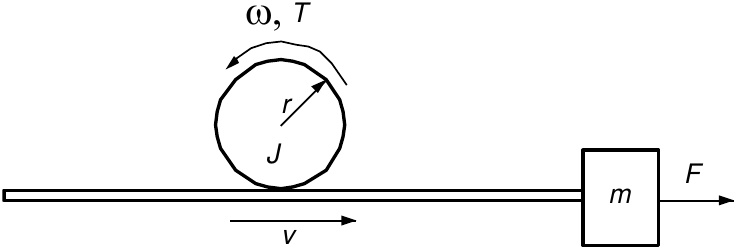
\includegraphics[width = 1\linewidth]{img/1/convertion.png} \label{fig:convertion}
    \end{minipage}
    \hfill
    \raisebox{0.75em}{\begin{minipage}{0.33\linewidth}\resizebox{0.55\hsize}{!}{$%
        \left\{
        \begin{aligned}
            v &= \omega r \\ 
            F &= \frac{1}{r} T
        \end{aligned}
        \right.
    $}
    \end{minipage}}
\end{figure}
\end{theo}

%//==============================--@--==============================//%
\newpage
\subsubsection[2.2.3 Motor Corrente Contínua]{$\pmb{\rightarrow}$ Motor de Corrente Contínua}
\mdfsetup{linewidth=2pt}
\begin{mdframed}
\textbf{Modelo do servomotor CC de íman permanente:}

\noindent\underline{Binário do motor}: Para um fluxo constante

\noindent \hspace*{1.5 em}\raisebox{0.2 em}{$\drsh$} $T(t) = K_T\, i(t)$

\vspace{0.5em}
\noindent\underline{Tensão aos terminais do rotor}: 

\noindent \hspace*{1.5 em}\raisebox{0.2 em}{$\drsh$} $e = K_e\, \omega$
%adoro-te :3 miminhooooooooooooooooooooooooooooooooooooooos

% cutie :3 -><- aaaaaaadoro-te
\end{mdframed}
\paragraph[2.2.3.1 Problema 1]{$\pmb{\star}$ Escreva as equações que modelam o sistema na forma de um modelo de estado (sistema
de equações diferenciais de 1ª ordem)}\mbox{}\\
\begin{figure}[H]
    \centering
    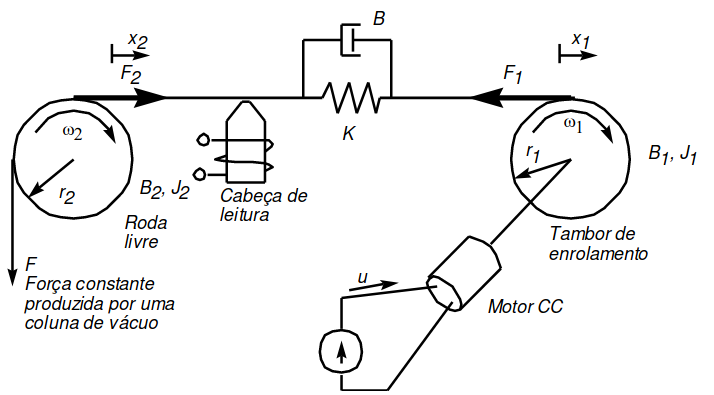
\includegraphics[width = 0.6\linewidth]{img/1/motor-cc-P16.png}
    \caption{P16 retirado da coletânea de exercícios.}
    \label{fig:motor-cc-P16}
\end{figure}

\noindent\underline{T. de Enrolamento}: de acordo com as equações subjacentes à mecânica de rotação

\noindent \hspace*{1.5 em}\raisebox{0.2 em}{$\drsh$} $J_1 \dot{\omega_1} = - F_1 r_1 - \beta_1 \omega_1 + T_{cc}$

\vspace{0.5em}
\noindent\underline{Roda Livre}: novamente, de acordo com as equações subjacentes à mecânica de rotação 

\noindent \hspace*{1.5 em}\raisebox{0.2 em}{$\drsh$} $J_1 \dot{\omega_2} = (F_2 - F) r_2 - \beta_2 \omega_2$

\vspace{0.5em}
\noindent\underline{Fita}: (\textit{vide} \hyperref[def:MolasElásticas]{secção das molas elásticas})

\noindent \hspace*{1.5 em}\raisebox{0.2 em}{$\drsh$} $
                \begin{cases}
                    F_1 = K(x_1 - x_2) + \beta(\dot{x_1} - \dot{x_2})\\
                    F_2 = -K(x_2 - x_1) - \beta(\dot{x_2} - \dot{x_1})\\
                \end{cases}
$

\vspace{0.5em}
\noindent\underline{Motor CC}: $T_{cc}$ é o binário exercido pelo motor CC no Tambor de Enrolamento

\noindent \hspace*{1.5 em}\raisebox{0.2 em}{$\drsh$} $T_{cc} = K_T\, u$

\vspace{0.5em}
\noindent\underline{Variáveis do referencial}: a velocidade linear de um ponto da periferia de uma roda é o produto do raio da roda pela velocidade angular

\noindent \hspace*{1.5 em}\raisebox{0.2 em}{$\drsh$} $
                \begin{cases}
                    \dot{x_1} = \omega_1 r_1\\
                    \dot{x_2} = \omega_2 r_2\\
                \end{cases}
$

%//==============================--@--==============================//%
\clearpage
\paragraph[2.2.3.2 Problema 2]{$\pmb{\star}$ Escreva as equações que modelam o sistema e um modelo de estado na forma de um sistema de
equações diferenciais de 1ª ordem.}\mbox{}\\
\begin{figure}[H]
    \centering
    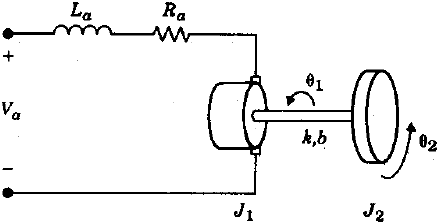
\includegraphics[width = 0.45\linewidth]{img/1/motor-cc-P18.png}
    \caption{P18 retirado da coletânea de exercícios. Motor elétrico que reboca uma carga com um modo dominante de vibração.}
    \label{fig:motor-cc-P18}
\end{figure}

\noindent \underline{Motor:} por aplicação da Lei das Malhas (KVL)

\noindent \hspace*{1.5 em}\raisebox{0.2 em}{$\drsh$} \textbf{KVL:} $ L_a \dfrac{d i_a}{dt} + i_a R_a + e_a - V_A = 0 \iff \dfrac{d i_a}{dt} = -\dfrac{K_e}{L_a} \dot{\theta}_1 - \dfrac{R_a}{L_a} i_a + V_A$

\vspace{0.5em}
\noindent \underline{Veio:} com as equações subjacentes à mecânica de rotação

\noindent \hspace*{1.5 em}\raisebox{0.2 em}{$\drsh$} $J_1 \ddot{\theta}_1 = -K(\theta_1 - \theta_2) -\beta(\dot{\theta}_1 - \dot{\theta}_2) + T_{cc}$

\vspace{0.5em}
\noindent\underline{Motor CC}: $T_{cc}$ é o binário exercido pelo motor CC no veio

\noindent \hspace*{1.5 em}\raisebox{0.2 em}{$\drsh$} $T_{cc} = K_T\, i_a$

\vspace{0.5em}
\noindent \underline{Carga:} de acordo com as equações subjacentes à mecânica de rotação

\noindent \hspace*{1.5 em}\raisebox{0.2 em}{$\drsh$} $J_2 \ddot{\theta}_2 = -K(\theta_2 - \theta_1) -\beta(\dot{\theta}_2 - \dot{\theta}_1)$

\vspace{0.5em}
\noindent Definem-se então os estados: $\pmb{x} = \begin{bmatrix} \theta_2 & \dot{\theta}_2 & \theta_1 & \dot{\theta}_1 & i_a\end{bmatrix}^T$

$$
    \therefore \dot{\pmb{x}} = 
    \begin{bmatrix} 
        0 & 1 & 0 & 0 & 0\\[4pt]
        -\frac{K}{J_2} & -\frac{\beta}{J_2} & \frac{K}{J_2} & \frac{\beta}{J_2} & 0\\[4pt]
        0 & 0 & 0 & 1 & 0\\[4pt]
        \frac{K}{J_1} & \frac{\beta}{J_1} & -\frac{K}{J_1} & -\frac{\beta}{J_1} & K_T\\[4pt]
        0 & 0 & 0 & -\frac{K_e}{L_a} & -\frac{R_a}{L_a}
    \end{bmatrix}
    \pmb{x} +
    \begin{bmatrix} 
        0\\
        0\\
        0\\
        0\\
        -\frac{1}{L_a}
    \end{bmatrix}
    V_A
$$

%//==============================--@--==============================//%
\clearpage
\paragraph[2.2.3.3 Problema 3]{$\pmb{\star}$ Defina um estado apropriado com a menor dimensão possível e escreva as respetivas equações de estado na forma matricial.}\mbox{}\\
\begin{figure}[H]
    \centering
    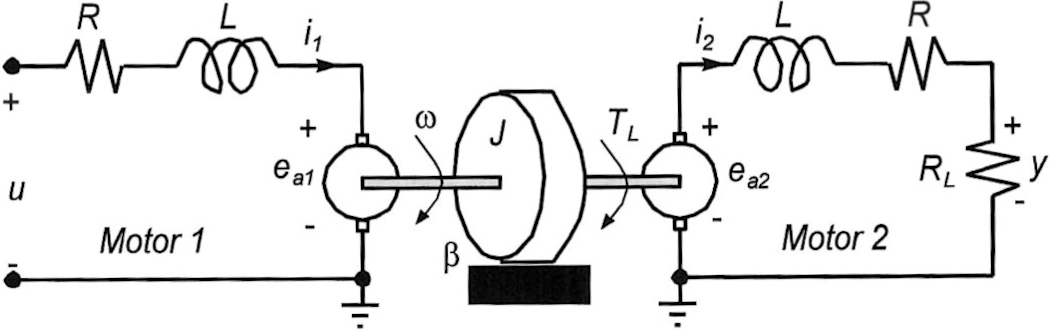
\includegraphics[width = 0.6\linewidth]{img/1/motor-cc-exame2021.png}
    \caption{Circuito eletromecânico equivalente de dois motores de corrente contínua de íman permanente, que têm os veios ligados solidariamente. $T_L = K_T\, i_1$ e $e_{ai} = K_{ei}\, \omega$}
    \label{fig:motor-cc-exame20/21}
\end{figure}

\noindent \underline{Motor 1:} por aplicação da Lei das Malhas (KVL)

\noindent \hspace*{1.5 em}\raisebox{0.2 em}{$\drsh$} \textbf{KVL:} $i_1 R + L \dfrac{d i_1}{dt} + e_{a1} - u = 0 \iff \dfrac{d i_1}{dt} = - \dfrac{R}{L} i_1 - \dfrac{K_{e1}}{L} \omega + \dfrac{1}{L}u$

\vspace{0.5em}
\noindent \underline{Motor 2:} por aplicação, novamente, da Lei das Malhas (KVL)

\noindent \hspace*{1.5 em}\raisebox{0.2 em}{$\drsh$} \textbf{KVL:} $L \dfrac{d i_2}{dt} + i_2 R + i_2 R_L - e_{a2} = 0 \iff \dfrac{d i_2}{dt} = \dfrac{K_{e2}}{L}\omega - \left(\dfrac{R+R_L}{L}\right) i_2$

\vspace{0.5em}
\noindent \underline{Roda:} de acordo com as equações subjacentes à mecânica de rotação

\noindent \hspace*{1.5 em}\raisebox{0.2 em}{$\drsh$} $J \dot{\omega} = T_L - \beta \omega \iff \dot{\omega} = -\dfrac{\beta}{J}\omega + \dfrac{K_T}{J} i_1$

\vspace{0.5em}
\noindent Definem-se então os estados: $\pmb{x} = \begin{bmatrix} \omega & i_1 & i_2 \end{bmatrix}^T$

$$
    \therefore \dot{\pmb{x}} = 
    \begin{bmatrix} 
        -\frac{\beta}{J} & \frac{K_T}{J} & 0\\[5pt]
        -\frac{K_{e1}}{L} & -\frac{R}{L} & 0\\[5pt]
        \frac{K_{e2}}{L} & 0 & \frac{K_T}{J}
    \end{bmatrix}
    \pmb{x} +
    \begin{bmatrix} 
        0\\[5pt]
        \frac{1}{L}\\[5pt]
        0
    \end{bmatrix}
    u,\qquad y = 
    \begin{bmatrix}
        0 & 0 & R_L
    \end{bmatrix}
    \pmb{x}
$$

%//==============================--@--==============================//%
        
    \clearpage
    \section{Resposta dinâmica}\label{sec:resposta-dinâmica}%
    %//==============================--@--==============================//%
\subsection[2.1 Resposta no Tempo]{\hspace*{0.075 em}\raisebox{0.2 em}{$\pmb{\drsh}$} Resposta no Tempo}
\label{sec:resposta-no-tempo}

\begin{theo}[\underline{Def.:} Função de transferência]{def:ft}\label{def:ft}
    \noindent ``The transfer function can be formally defined as follows: The function, which is the transfer gain from $U(s)$ to $Y(s)$ --- input to output --- is called the transfer
    function of the system. It is the ratio of the Laplace transform of the output of the
    system to the Laplace transform of the input.

    $$
        \dfrac{Y(s)}{U(s)} = F(s)
    $$
    \noindent with the key assumption that all of the initial conditions on the system are zero."\cite{FranklinPowell2015}
\end{theo}

\noindent A função de transferência é um conceito potente:

\begin{itemize}
    \item não depende nem da entrada nem da saída do sistema
    \item caracteriza completamente o sistema do ponto de vista de entrada-saída
\end{itemize}

$$
     F(s) = \dfrac{Y(s)}{U(s)} = \dfrac{\text{polinómio de grau m}}{\text{polinómio de grau n}}
$$

\begin{itemize}
    \item n > m a função de transferência diz-se estritamente própria
    \item n $\ge$ m a função de transferência diz-se prória
    \item n < m a função de transferência diz-se imprópria
\end{itemize}

\noindent ``The roots of the denominator $U(s)$, $\{p_1,p_2,\dots,p_n\}$, are called the poles of the system.
The poles are locations in the s-plane where the magnitude of the transfer function becomes infinite if $s = p_i$:

$$
    \boxed{|F(s)|_{s = p_i} = \infty}
$$

\noindent The roots of the numerator, $Y(s)$, $\{z_1,z_2, \dots, z_n\}$ are called the finite zeros of the system. The zeros are locations in the s-plane where the transfer function is zero. If $s = z_i$:"\cite{FranklinPowell2015}

$$
    \boxed{|F(s)|_{s = z_i} = 0}
$$

\noindent A sua interação influência a característica da resposta do sistema:

{\setlength{\tabcolsep}{16pt}
\begin{center}
    \begin{tabular}{p{0.4\textwidth} | p{0.4\textwidth}}
        \centerline{\underline{$\#\textbf{pólos} > \#\textbf{zeros}$}} & \centerline{\underline{$\#\textbf{pólos} > \#\textbf{zeros}+1$}} \\[-14pt]
        Resposta ao escalão contínua & Derivada da resposta contínua \\[4pt]
        \centerline{\underline{$\#\textbf{pólos} = \#\textbf{zeros}$}} & \centerline{\underline{$\#\textbf{pólos} = \#\textbf{zeros}+1$}} \\[-14pt]
        Resposta descontínua, com salto finito & Derivada da resposta descontínua, mas finita \\[4pt]
        \centerline{\underline{$\#\textbf{pólos} < \#\textbf{zeros}$}} & \centerline{\underline{$\#\textbf{pólos} < \#\textbf{zeros}+1$}} \\[-14pt]
        Resposta descontínua, com salto infinito & Derivada da resposta descont.,  infinita \\
        \bottomrule
    \end{tabular}
\end{center}
}

\newpage
\subsubsection[2.1.1 Análise da função de transferência]{$\pmb{\rightarrow}$ Análise da função de transferência}

Se $f(t)$ não contiver impulsos ou singularidades de ordem superior na origem e convergir para um valor constante quando $t \to +\infty$, então, aplicam-se os teoremas:
\begin{center}%
    \begin{tabular}{c c}%
        \begin{minipage}{0.425\linewidth}%
            \begin{theo}[\underline{Teorema do Valor Incial}]{teo:inicial-value}\label{teo:inicial-value}
                $$
                    \lim_{t \to 0} f(t) = \lim_{s \to +\infty} sF(s)
                $$
            \end{theo}%
        \end{minipage}%
        &%
        \begin{minipage}{0.425\linewidth}%
            \begin{theo}[\underline{Teorema do Valor Final}]{teo:final-value}\label{teo:final-value}
                $$
                    \lim_{t \to +\infty} f(t) = \lim_{s \to 0} sF(s)
                $$
            \end{theo}%
        \end{minipage}%
    \end{tabular}%
\end{center}%

\subsubsection[2.1.2 Resposta ao escalão unitário de sistemas LIT]{$\pmb{\rightarrow}$ Resposta ao escalão unitário de sistemas LIT}

\begin{figure}[H]
    \centering
    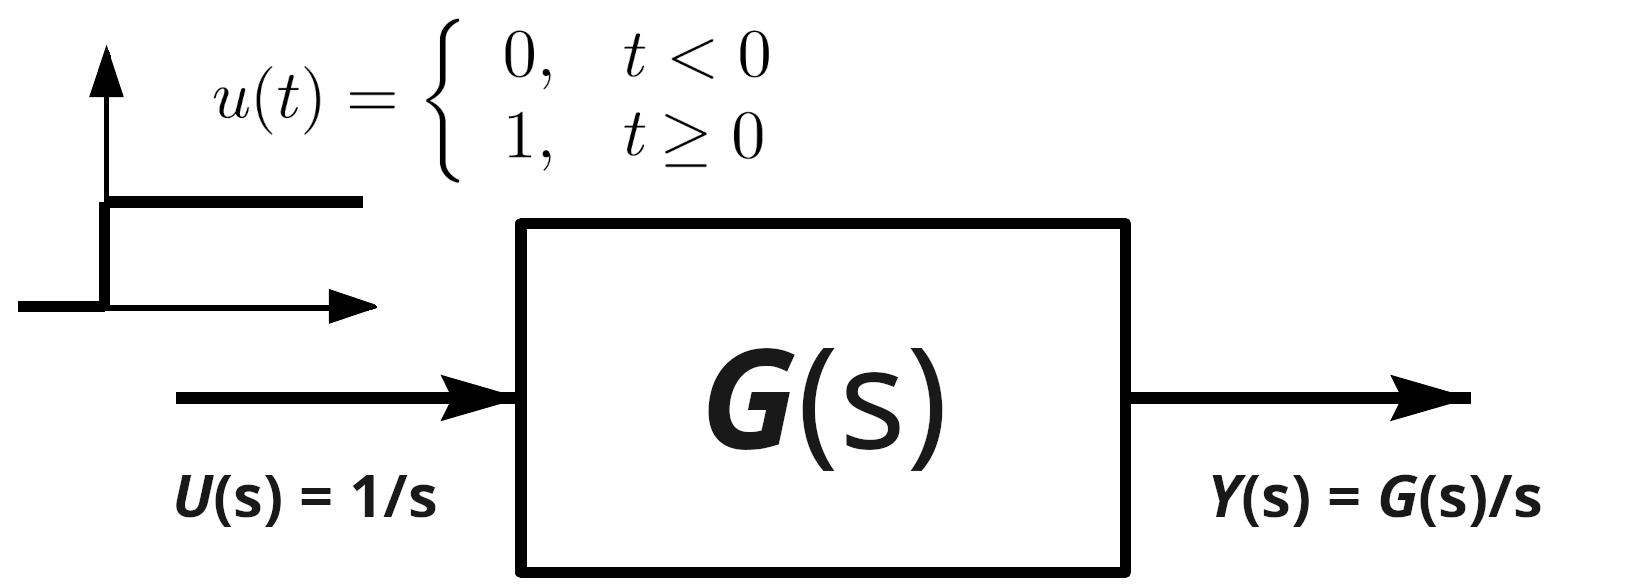
\includegraphics[width = 0.5\linewidth]{img/2/unit-step-response.png}
    \caption{Resposta do sistema ao degrau unitário.}
    \label{fig:unit-step-response}
\end{figure}

{
\mdfsetup{linewidth=2pt}

\begin{mdframed}
    \begin{itemize}
    \item[$\blacktriangle$] \underline{Valor final da resposta} ao escalão unitário:
        
        \vspace{-1em}
        $$
            \lim_{t \to +\infty} y(t) = \lim_{s \to 0} sY(s) = \lim_{s \to 0} s\frac{G(s)}{s} = G(0)
        $$
        
    \vspace{-0.5em}
    \item[$\blacktriangle$] \underline{Valor inicial da resposta} ao escalão:
        
        \vspace{-1em}
        $$
            \lim_{t \to 0} y(t) = \lim_{s \to +\infty} sY(s) = \lim_{s \to +\infty} s\frac{G(s)}{s} = \lim_{s \to +\infty} G(s)
        $$
        
    \vspace{-0.5em}
    \item[$\blacktriangle$] \underline{Valor inicial da derivada da resposta} ao escalão unitário:
        
        \vspace{-1em}
        $$
            \lim_{t \to 0} \dot{y}(t) = \lim_{s \to +\infty} s\, (sY(s)) = \lim_{s \to +\infty} s^2\frac{G(s)}{s} = \lim_{s \to +\infty} sG(s)
        $$

    \vspace{-0.5em}
    \item[$\blacktriangle$] \underline{Valor final da derivada da resposta} ao escalão unitário:
        
        \vspace{-1em}
        $$
            \lim_{t \to +\infty} \dot{y}(t) = \lim_{s \to 0} s\, (sY(s)) = \lim_{s \to 0} s^2\frac{G(s)}{s} = \lim_{s \to 0} s G(s)
        $$
    \end{itemize}
\end{mdframed}
}
\paragraph[2.1.2.1 Sistema de 1º ordem]{$\pmb{\star}$ Sistema de 1º ordem:} Seja $G(s)$ a função de transferência de um sistema de primeira ordem em resposta ao escalão unitário:
$$
    G(s) = K_0 \cdot \dfrac{a}{s + a} 
$$
\noindent \textbf{Ganho estático}: O ganho estático, $K_0 = G(0)$, denomina o rácio da relação entre entrada e saída do sistema, na análise \textit{steady state}. 

\vspace{1 em}
\noindent \textbf{Tempo de estabelecimento:} Tempo ao fim do qual a resposta se confina a uma faixa de $\pm x\%,\;\, x \in \{2,3,5,7,\dots\}$
\begin{align*}
    Y(s) &= G(s)U(s)\;\; \overset{\mathcal{L}}{\Longrightarrow}\;\; K_0 (1 - e^{-at}),\;\, t \ge 0\\[4pt]
    t_s &= \dfrac{-\ln(0.02)}{a} \simeq \dfrac{4}{a} = 4\tau
\end{align*}

\noindent Onde $\tau = \frac{1}{a}$ é a constante de tempo do sistema, que denota o tempo necessário para que a resposta ao grau unitário atinga 63\% do seu valor final.

\paragraph[2.1.2.2 Sistema de 2º ordem]{$\pmb{\star}$ Sistema de 2º ordem:} Seja $G(s)$ a função de transferência de um sistema de segunda ordem em resposta ao escalão unitário:
$$
    G(s) = \dfrac{w_n^2}{s^2 + \zeta w_n s + w_n^2} 
$$

\begin{mdframed}
\noindent A resposta do sistema ao degrau unitário está totalmente dependente da localização dos pólos:
$$
    s^2 + \zeta w_n s + w_n^2\;\; \Longrightarrow\;\; s = -\zeta w_n \pm w_n\sqrt{\zeta^2 - 1}
$$

\begin{itemize}
    \item \textbf{Sistema subamortecido:} $0 \ge \zeta < 1$
    $$
        \boxed{s = -\zeta w_n \pm j w_n\sqrt{1 - \zeta^2}}
    $$
    \item \textbf{Sistema criticamente amortecido:} $\zeta = 1$
    $$
        \boxed{s = -w_n}
    $$
    \item \textbf{Sistema sobreamortecido:} $\zeta > 1$
    $$
        \boxed{s = -\zeta w_n \pm w_n\sqrt{\zeta^2 - 1}}
    $$
\end{itemize}

\noindent \textbf{Nota:} Os parâmetros acima mencionados possuem a seguinte nomenclatura:

\begin{itemize}
    \item Frequência das oscilações naturais sem amortecimento, $w_n$
    \item Coeficiente de amortecimento, $\zeta$
    \item Frequência das oscilações amortecidas, $w_d = w_n\sqrt{\zeta^2 - 1}$
\end{itemize}
\end{mdframed}

\vspace{-2em}
\begin{figure}[H]
    \centering
    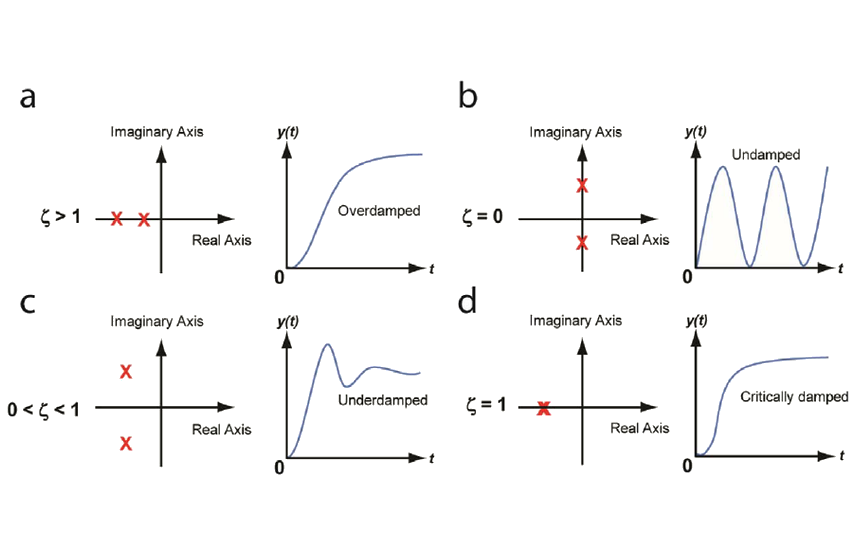
\includegraphics[width = 0.8\linewidth]{img/2/second-order-system.png}
    \caption{Tipos de respostas de sistemas de segunda ordem sem zeros}
    \label{fig:LABEL}
\end{figure}

%//==============================--@--==============================//%
\subsubsection[2.1.3 Especificações do domínio do tempo]{$\pmb{\rightarrow}$ Especificações do domínio do tempo}

\noindent As especificações de desempenho para um projeto de sistema de controle frequentemente envolvem certos requisitos associados à resposta do tempo do sistema. Os requisitos para uma resposta ao degrau unitário são expressos em termos das quantidades padrão:

\begin{itemize}
    \item \textbf{Tempo de crescimento}, \textit{rise time}, $t_r$ tempo que o sistema leva para atingir a proximidade do seu novo ponto de ajuste.
    \item \textbf{Tempo de pico}, \textit{peak time}, $t_p$ é o tempo que o sistema leva a atingir o ponto máximo de sobreelevação.
    \item \textbf{Tempo de estabelecimento}, \textit{setting time}, $t_s$ é o tempo que o sistema leva para transitar para o regime estacionário.
    \item \textbf{Sobreelevação}, \textit{overshoot}, $M_p$ é a quantidade máxima que o sistema ultrapassa o seu valor final, dividido pelo seu valor final (usualmente expresso em percentagem)
\end{itemize}

\paragraph[2.1.3.1 Rise time]{$\pmb{\star}$ Rise time}\mbox{}

\noindent Par um sistema de segunda ordem se zeros, o  \textit{rise time} é dado por:
$$
\boxed{t_r = \dfrac{1.8}{w_n}}
$$
\noindent ``It is accurate only for a second-order system with no zeros; for all other systems, it is a rough approximation to the relationship between $t_r$ and $w_n$."\cite{FranklinPowell2015}

\paragraph[2.1.3.2 Tempo de pico]{$\pmb{\star}$ Tempo de pico}\mbox{}\\

\noindent O tempo de pico é obtido quando se anula a derivada da resposta no tempo do sistema ao grau unitário. Tomando o modelo de segunda ordem sem zeros já acima mencionado:

$$
    y(t) = 1 - e^{-\sigma t}\left(cos w_d t + \dfrac{\sigma}{w_d}\sin w_d t\right),\;\, \sigma = \zeta w_n
$$

A equação acima pode ser reescrita recorrendo à seguinte entidade trigonomérica:
$$
    A\sin(\alpha) + Bcos(\alpha) = C\cos(\alpha - \beta)
$$

\noindent O que resulta na seguinte forma compacta:
$$
    y(t) = 1 - \dfrac{e^{\sigma t}}{\sqrt{1 - \zeta}}\left(\cos{w_d t - \beta}\right)
$$

\noindent A respetiva derivada possui a seguinte forma:
$$
    \dot{y}(t) = e^{-\sigma t}\left(\dfrac{\sigma^2}{w_d} + w_d\right)\sin{w_d t}
$$

\noindent A derivada anula-se para:
$$
    w_d t_p = \pi
$$

\noindent Logo, podemos definir o tempo de pico como:
$$
    \boxed{t_p = \dfrac{\pi}{w_d}}
$$

\paragraph[2.1.3.4 Sobreelevação]{$\pmb{\star}$ Sobreelevação}\mbox{}\\

\noindent A sobreelevação é obtida através da aplicação do resultado previamente obtido na expressão de $y(t)$.
$$
    \boxed{\dfrac{y_{\textit{máx}} - y_{min}}{y_{final}} = M_p = e^{-\pi \zeta / \sqrt{1 - \zeta^2}}}
$$

\paragraph[2.1.3.3 Tempo de estabelecimento]{$\pmb{\star}$ Tempo de estabelecimento}\mbox{}\\

\noindent O tempo de estabelecimento, como já explicictado no sistema de 1ª ordem, é o instante de tempo em que a saída atinge e se mantém numa faixa de $\pm 2\%$ do valor final:

$$
    y(t) = 1 - e^{-\sigma t}\left(cos w_d t + \dfrac{\sigma}{w_d}\sin w_d t\right),\;\, \sigma = \zeta w_n
$$

\noindent ``As an analytic computation, we notice that the deviation of from 1 is the product of the decaying exponential, $e^{-\sigma t}$, and the circular functions sine and cosine. The duration of this error is essentially decided by the transient exponential, so we can define the settling time as
that value of $t_s$ when the decaying exponential reaches $1\%$ (or any other number for that matter, tipically we use $2\%, 5\%, 7\%, \dots$):

$$
    \begin{aligned}
        &e^{\sigma t_s} = 0.01\\
        &t_s = \dfrac{\ln{0.01}}{\sigma} \simeq \dfrac{4.6}{\sigma}
    \end{aligned}
$$

\begin{center}
    \begin{minipage}{0.45\textwidth}
        \begin{itemize}[leftmargin=*]
        \item[] \textbf{\emph{Coeficiente de amortecimento}}: O coeficiente é constante em cada uma das retas apresentadas. Quanto maior for o coeficiente, menor é o \textit{overshoot}.
        \end{itemize}
    \end{minipage}%
    \hfill
    \begin{minipage}{0.55\textwidth}
        \begin{center}
            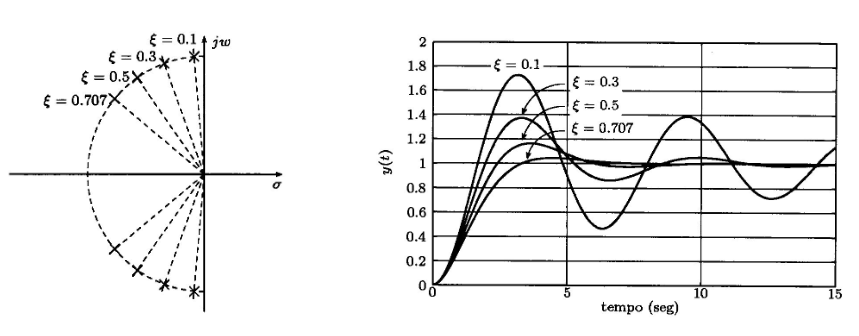
\includegraphics[width=0.95\textwidth]{img/2/overshoot.png}
            \label{img:overshoot}
        \end{center}
    \end{minipage}
\end{center}

\begin{center}
    \begin{minipage}{0.45\textwidth}
        \begin{itemize}[leftmargin=*]
        \item[] \textbf{\emph{Oscilações amortecidas}}: O pa- râmetro $\sigma$ é constante na continuidade da reta apresentada. Quanto maior for $w_d$, menor é o \textit{peak time}.
        \end{itemize}
    \end{minipage}%
    \hfill
    \begin{minipage}{0.55\textwidth}
        \begin{center}
            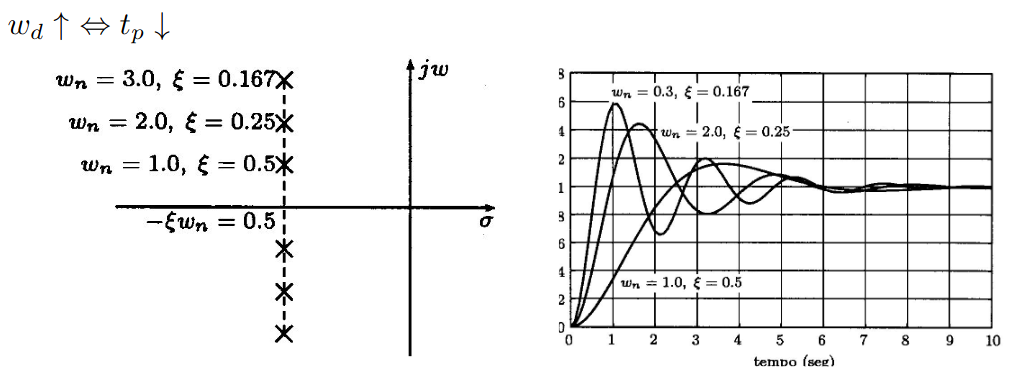
\includegraphics[width=1\textwidth]{img/2/peak-time.png}
            \label{img:peak-t}
        \end{center}
    \end{minipage}
\end{center}

\begin{center}
    \begin{minipage}{0.45\textwidth}
        \begin{itemize}[leftmargin=*]
        \item[] \textbf{\emph{Parâmetro $\mathbf{\sigma}$}}: O parâmetro $w_d$ é constante na continuidade da reta horizontal apresentada. Quanto maior for $\sigma$, menor é o \textit{setting time}.
        \end{itemize}
    \end{minipage}%
    \hfill
    \begin{minipage}{0.55\textwidth}
        \begin{center}
            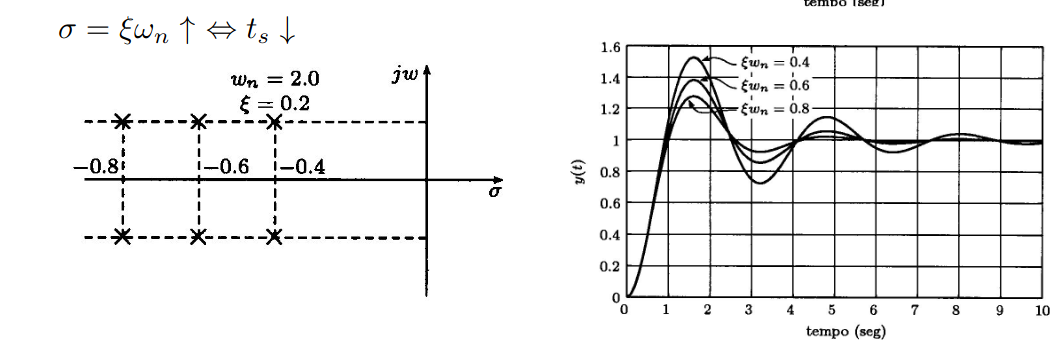
\includegraphics[width=1\textwidth]{img/2/setting-time.png}
            \label{img:set-time}
        \end{center}
    \end{minipage}
\end{center}

%//==============================--@--==============================//%
\newpage
\subsubsection[2.1.3 Influência de pólos e zeros adicionais]{$\pmb{\rightarrow}$ Influência de pólos e zeros adicionais}

\noindent Supondo o seguinte sistema de ordem superior:
$$
    H(s) = \dfrac{25 \cdot a}{(s + a)(s^2 + 4s + 25)}
$$
\noindent  ``The additional pole will contribute more damping to the system response. This will reduce the Percent Overshoot, but at the same time, it will slow the system response increasing Rise Time and Settling Time. Since \textbf{each additional pole contributes an additional exponential term that must die out before the system
reaches its final value}, each additional pole increases the rise time of the system"\cite{FranklinPowell2015} 

\vspace{1 em}
\noindent Quando $|a|$ aumenta
\begin{itemize}
    \item a influência do pólo diminui
    \item O pólo torna-se “menos dominante”
    \item Os pólos complexos tornam-se pólos dominantes
\end{itemize}

\noindent É possível aproximar o sistema de um de segunda ordem (desprezar o pólo não dominante) quando:
\begin{itemize}
    \item Quando o regime transitório associado é desprezável, no conjunto de todas as
contribuições transitórias, ao fim de aproximadamente 5 constantes de tempo.
    \item Quando o módulo do pólo real é pelo menos cinco vezes maior que o módulo
da parte real dos pólos dominantes.
\end{itemize}

\noindent Suponhamos agora os seguinte sistemas:
$$
    \begin{aligned}
        H_1(s) &= \dfrac{2}{(s + 1)(s + 2)} = \dfrac{2}{s + 1} + \dfrac{2}{s + 2}\\[4pt]
        H_2(s) &= \dfrac{2(s + 1.1)}{1.1 (s + 1)(s + 2)} = \dfrac{0.18}{s + 1} + \dfrac{1.64}{s + 2}
    \end{aligned}
$$
\noindent O coeficiente do termo $(s + 1)$ sofreu uma redução drástica com a introdução de um zero na sua periferia (como seria de esperar, se o pólo e o zero possuirem o mesmo termo, a influência do pólo é totalmente anulada). Assim, de forma geral, \textbf{``a zero near a pole reduces the amount of that term in the total response."}\cite{FranklinPowell2015}

\vspace{1 em}
\noindent Neste sentido, a introdução de um zero no semiplano complexo esquerdo (spce) torna o sistema mais rápido (diminuição do tempo de estabelecimento e \textit{rise time}) e aumenta a sobreelevação. Na mesma sequência, a introdução de um zero no semiplano complexo direito (spcd) torna o sistema mais lento e introduz \textit{undershoot} (já que o termo derivativo da resposta no tempo passa a ser subtraído). Sistemas como estes denominam-se \textbf{sistemas de fase não mínima}:

$$
    H(s) = \dfrac{s - 1}{s^2 + s + 1} 
$$

\newpage
{
\mdfsetup{linewidth=2pt}

\begin{mdframed}
    \noindent\textbf{Resumo:}
    \begin{itemize}
        \item Adding a LHP zero to the transfer function makes the step response faster (decreases the rise time
and the peak time) and increases the overshoot.
        \item Adding a RHP zero to the transfer function makes the step response slower, and can make the
response undershoot.
        \item Adding a LHP pole to the transfer function makes the step response slower.
    \end{itemize}

    \noindent Aproximação por sistemas de ordem mais baixa:
    \begin{itemize}
        \item A resíduo associado ao pólo é pequeno (está próximo de um zero) $\rightarrow$ despreza-se o pólo e o zero.
        \item A parte real do pólo é elevada (e portanto possui um regime transitório desprezável) $\rightarrow$ despreza-se o pólo.
    \end{itemize}

    \noindent\textbf{Nota:} O sistema original e o aproximado devem ter o mesmo ganho estático
\end{mdframed}
}

%//==============================--@--==============================//%
    %//==============================--@--==============================//%
\subsection[2.2 Estabilidade]{\hspace*{0.075 em}\raisebox{0.2 em}{$\pmb{\drsh}$} Estabilidade}
\label{sec:stability}

\begin{theo}[\underline{Def.:} Estabilidade]{def:ft}\label{def:stability}
    \noindent ``An LTI system is said to be stable if all the roots of the transfer function denominator polynomial have negative real parts (that is, they are all in the left hand s-plane), and is unstable otherwise."\cite{FranklinPowell2015}
\end{theo}

%//==============================--@--==============================//%
\subsubsection[2.2.1 Bounded input Bounded output (BIBO)]{$\pmb{\rightarrow}$ Bounded input Bounded output (BIBO)}

\noindent SLIT é BIBO (Bounded Input Bounded Output) estável: Qualquer sinal de entrada limitado conduz a um sinal de saída limitado. Considerando um SLIT com input $u(t)$ e output $y(t)$:

$$
    y(t) = \int_{-\infty}^{+\infty} h(\tau)u(t - \tau)d\tau
$$
\noindent Se $u(t)$ for $bounded$, de forma a que exista uma constante $M$ tal que $|u(t)| \leq M \leq \infty$, $y(t)$ será $bounded$ da seguinte forma:

$$
    \begin{aligned}
        |y| &= \left|\int h u d\tau\right|\\
        &\leq \int |h| |u| d\tau\;\; \rightarrow\;\; \text{desigualdade triangular}\\
        &\leq M\int |h|d\tau < \infty
    \end{aligned}
$$

\begin{theo}[\underline{Def.:} Estabilidade BIBO]{def:ft}\label{def:stability_BIBO}
    \noindent ``The system with impulse response $h(t)$ is BIBO-stable
if and only if the integral"\cite{FranklinPowell2015}

    $$
        \int |h|du < \infty
    $$
\end{theo}

%//==============================--@--==============================//%
\subsubsection[2.2.2 Estabilidade de um SLIT]{$\pmb{\rightarrow}$ Estabilidade de um SLIT}

\noindent Um sistema SLIT é estável se e só se (condição necessária e suficiente) todos os termos da resposta no tempo tendam para zero enquanto $t \to \infty$.
$$
    e^{p_i t} \to 0,\;\, \text{para todos os $p_i$}
$$

\noindent Tal acontece se
$$
    \boxed{\text{Re}\{p_i\} < 0}
$$

\noindent ``This is called. internal stability. Therefore, \textbf{the stability of a system can be determined by computing the location of the roots} of the characteristic equation and determining whether they are all in the LHP."\cite{FranklinPowell2015} Logo, o eixo imaginário é uma barreira de estabilidade.

\paragraph[2.2.2.1 Estabilidade Marginal]{$\pmb{\star}$ Estabilidade Marginal}\mbox{}\\

\noindent Considerando o seguinte sistema que possui dois pólos puramente imaginários:
$$
    \dfrac{4}{s^2 + 4}\quad p_{1,2} = \pm j2
$$

\noindent A resposta ao degrau unitário deste sistema é:
$$
  y(t) = 1 - \cos{(2t)}
$$

\begin{itemize}
    \item O sistema oscila indefinidamente, já que $\zeta = 0$.
    \item O sistema é \textbf{marginalmente estável}: a resposta natural nem cresce nem se atenua, permanecendo constante ou oscilante, à medida que o tempo tende para o infinito.
\end{itemize}

\noindent Considerando agora o seguinte sistema que possui quatro pólos puramente imaginários repetidos:
$$
    \dfrac{16}{(s^2 + 4)^2}\quad p_{1,2} = \pm j2\quad p_{3,4} = \pm j2
$$

\noindent A resposta ao degrau unitário deste sistema é:
$$
  y(t) = 1 - \cos{(2t)} - t\sin{(2t)}
$$

\begin{itemize}
    \item O sistema cresce sem \textit{bound} graças ao segundo termo da resposta natural do sistema $t\sin{(2t)}$.
    \item O sistema é instável.
    \item Múltiplos pólos imaginários repetidos no eixo imaginário pressupõe um sistema instável.
\end{itemize}

\paragraph[2.2.2.1 Critério de Routh-Hurwitz]{$\pmb{\star}$ Critério de Routh-Hurwitz}

{
\mdfsetup{linewidth=2pt}

\begin{mdframed}
\textbf{Critério de Hurwitz} uma condição necessária (mas não suficiente) de estabilidade de um SLIT causal é que todos os coeficientes do polinómio denominador da FT sejam positivos (ou tenham o mesmo sinal).
\end{mdframed}
}

\noindent Esta condição é verficada por inspeção direta do polinómio característico do sistema.

\newpage
\noindent ``Once the elementary necessary conditions have been satisfied, we need a more powerful test. Routh’s formulation requires the computation of a \textbf{triangular array}".\cite{FranklinPowell2015} Supondo o seguinte polinómio característico de ordem $n$:

$$
    a(s) = s^n + a_1 s^{n - 1} + a_2 s^{n - 2} + \dots a_{n -1} s + a_n
$$

\noindent \textbf{1.} Para determinar a matriz de Routh, primeiro organizamos os coeficientes do polinómio característico em duas filas, começando com o primeiro e o segundo coeficiente2, seguidos dos coeficientes pares e ímpares:

$$
    \begin{aligned}
        s^n&: 1,\;\; a_2\;\; a_4\;\; \dots\\
        s^{n-1}&: a_1,\;\; a_3\;\; a_5\;\; \dots\\
    \end{aligned}
$$
\noindent\textbf{2.} De seguida, adicionamos as linhas subsequentes (correspondentes aos restantes coeficientes) para completar a matriz de Routh. Calculamos os elementos das linhas $s^{n - 2}$ e das linhas $s^{n - 3}$ da seguinte forma:

$$
    \begin{aligned}
        b_1 = -\dfrac{\begin{bmatrix}
                        1 & a_2\\
                        a_1 & a_3        
                    \end{bmatrix}}{a_1} = \dfrac{a_1 a_2 - a_3}{a_1}\quad
        c_1 = -\dfrac{\begin{bmatrix}
                        a_1 & a_3\\
                        b_1 & b_2        
                    \end{bmatrix}}{b_1} = \dfrac{b_1 a_3 - a_1 b_2}{b_1}\\
        b_2 = -\dfrac{\begin{bmatrix}
                        1 & a_4\\
                        a_1 & a_5        
                    \end{bmatrix}}{a_1} = \dfrac{a_1 a_4 - a_5}{a_1}\quad
        c_2 = -\dfrac{\begin{bmatrix}
                        a_1 & a_5\\
                        b_1 & b_3        
                    \end{bmatrix}}{b_1} = \dfrac{b_1 a_5 - a_1 b_3}{b_1}\\
        b_3 = -\dfrac{\begin{bmatrix}
                        1 & a_6\\
                        a_1 & a_7        
                    \end{bmatrix}}{a_1} = \dfrac{a_1 a_6 - a_7}{a_1}\quad
        c_3 = -\dfrac{\begin{bmatrix}
                        a_1 & a_7\\
                        b_1 & b_4        
                    \end{bmatrix}}{b_1} = \dfrac{b_1 a_7 - a_1 b_4}{b_1}
    \end{aligned}
$$

\noindent Note-se que os elementos das linhas subsequentes são formados a partir das duas linhas anteriores usando os determinantes da matrizes formadas pelos dois elementos da primeira coluna e os outros elementos das colunas sucessivas.

\vspace{1 em}
\noindent\textbf{3.} Por fim, verificamos se os elementos da primeira coluna são todos positivos. Se sim, então o sistema é estável, caso contrário, instável.
%//==============================--@--==============================//%

    \clearpage
    \section{Feedback analysis}
    %//==============================--@--==============================//%
\subsection[3.1 Equações básicas de Controlo ]{\hspace*{0.075 em}\raisebox{0.2 em}{$\pmb{\drsh}$} Equações básicas de Controlo}
\label{sec:eq-base-control}
\noindent Considerando o seguinte diagrama de blocos reunem-se de seguida um conjunta de equações com respeito aos sistemas de malha aberta e malha fechada:

\begin{figure}[H]
    \centering
    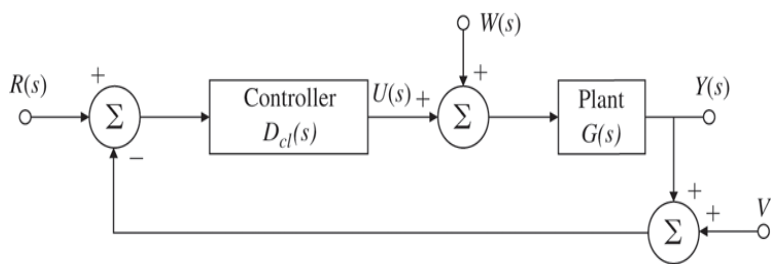
\includegraphics[width = 0.8\linewidth]{img/3/feedback-loop.png}
    \caption{diagrama de blocos generalista de um dado sistema}
    \label{fig:feed-loop}
\end{figure}

\noindent Supondo o sistema em \textbf{malha aberta}, podemos garantir a a equação de saída do sistema com recurso ao princípio da sobreposição. Neste sentido o sistema é linear com a seguinte saída:
$$
    Y_{ol} = G D_{ol} R - G W
$$
\noindent Onde $W$ são as perturbações induzidas pelo meio.

\vspace{1 em}
\noindent Consequentemente, a equação do erro, diferença entre a entrada de referência e a saída, é dada por:
$$
\begin{aligned}
    E_{ol} &= R - Y_{ol}\\
    &= R - G D_{ol} R - G W\\
    &= R[1 - G D_{ol}] - G W
\end{aligned}
$$

\noindent  função de transferência em cadeia aberta é portanto:
$$
    \boxed{T(s) = G(s) D_{ol}(s)}
$$

\noindent Supondo agora o sistema em \textbf{malha fechada}. Existem três entradas externas: a referência, $R$, que se espera que a saída siga; a perturbação do meio, $W$, que se espera que o controlo contrarie para não perturbar a saída; e o ruído do sensor, $V$, que se espera que o controlador ignore:
$$
\begin{aligned}
    Y_{cl} = \dfrac{GD_{cl}}{1 + GD_{cl}}R + \dfrac{G}{1 + GD_{cl}}W + \dfrac{GD_{cl}}{1 + GD_{cl}}V\\
    U_{cl} = \dfrac{D_{cl}}{1 + GD_{cl}}R + \dfrac{GD_{cl}}{1 + GD_{cl}}W + \dfrac{D_{cl}}{1 + GD_{cl}}V
\end{aligned}
$$

\noindent Onde o erro é novamente dado por $E_{cl} = R - Y_{cl}$ e a função de transferência é
$$
    \boxed{T(s) = \dfrac{D_{cl}}{1 + GD_{cl}}}
$$

%//==============================--@--==============================//%
\newpage
\subsection[3.2 Objectivos Gerais de um Sistema de Controlo]{\hspace*{0.075 em}\raisebox{0.2 em}{$\pmb{\drsh}$} Objectivos Gerais de um Sistema de Controlo}
\label{sec:obj-gerais-cont}

\begin{itemize}
\item Bom seguimento do sinal de referência --- a variável que se pretende controlar deve tomar valores tão próximos quanto possível dos valores desejados expressos pela referência, ou seja, o erro deve ser pequeno
\item Boa rejeição dos efeitos das perturbações, incluindo ruído
\item Rapidez da resposta, quer no seguimento, quer na rejeição de perturbações
\item Estabilidade
\item Pequena sensibilidade à variação de parâmetros
\item Robustez de estabilidade
\begin{itemize}
    \item Relativamente à variação de parâmetros
    \item Relativamente a incertezas no modelo do sistema físico no qual se baseou o projeto de controlador
\end{itemize}
\item Dinâmica não modelada, resultante, por exemplo, da aproximação de um sistema de 3ª ordem por um modelo mais simples de 2ª ordem
\end{itemize}

%//==============================--@--==============================//%
\subsubsection[3.2.1 Seguimento do sinal de referência]{$\pmb{\rightarrow}$ Seguimento do sinal de referência}
\noindent Se considerarmos apenas o seguimento da entrada de referência e definirmos $W = V = 0$ então a equação para o erro é simplesmente:

$$
    \dfrac{E}{R} = \dfrac{1}{1 + GD_{cl}}
$$
\noindent Considerando entradas polinomiais, admitimos que $R = \frac{1}{s^{k + 1}}$. Tomando um sistema mecânico como base para uma nomenclatura genérica de referência, chamamos às entradas em degrau para as quais $k = 0$, "posição", às entradas em rampa para as quais $k = 1$, "velocidade" e  às entradas para as quais $k = 2$, "aceleração. A aplicação do Teorema do Valor Final à fórmula de erro indica o seguinte resultado:

$$
    \begin{aligned}
        e_{ss} &= \lim_{s \to 0} s E(s)\\
        &= \lim_{s \to 0} \dfrac{s}{1 + GD_{cl}} \cdot \dfrac{1}{s^{k + 1}}
    \end{aligned}
$$

\noindent Consideramos primeiro um sistema para o qual não há pólo na origem, e uma entrada em degrau unitário para a qual $R(s) = \frac{1}{s}$. o limite acima descrito é reduzido para:
$$
    \lim_{s \to 0} \dfrac{s}{1 + GD_{cl}} \cdot \dfrac{1}{s} = \dfrac{1}{1 + GD_{cl}(0)} = \dfrac{1}{1 + K_p}
$$

\noindent Repare-se que a equação acima produz o erro estático de posição e que, se a entrada fosse um polinómio de grau superior a 1, o erro resultante cresceria sem limites. Um polinómio de grau 0 é o grau mais elevado que um sistema de tipo 0 pode seguir.

\vspace{1 em}
\noindent Supondo agora uma visão mais generalista, iremos escrever a função de transferência em malha aberta da seguinte forma:

$$
    GD_{cl} = \dfrac{GD_{clo}}{s^n}
$$
\noindent Se o sistema não possuir um pólo na origem então $n = 0$, se possuir um, $n = 1$, $\dots$

\noindent Assim, reescrevendo a equação do erro:
$$
    \begin{aligned}
        e_{ss} &= \lim_{s \to 0} s E(s)\\
        &= \lim_{s \to 0} \dfrac{s}{1 + \dfrac{GD_{clo}}{s^n}} \cdot \dfrac{1}{s^{k + 1}}\\
        &= \lim_{s \to 0} \dfrac{s^n}{s^n + K_N}\dfrac{1}{s^k}
    \end{aligned}
$$

\noindent Da equação acima, é fácil observar que se $n > k$ então $e_{ss} = 0$ e que se $n < k$ então $e_{ss} \to \infty$ e se $k = n \neq 0$, então $e_{ss} = 1/K_n$. Assim:

\begin{itemize}
    \item Se $n = k = 0$, $K_0 = K_p$ é denominada de "constante de posição", e o sistema é classificado como de tipo 0.
    \item Se $n = k = 0$, $K_1 = K_v$ é denominada de "constante de velocidade", e o sistema é classificado como de tipo 1.
    \item Se $n = k = 2$, $K_2 = K_a$ é denominada de "constante de aceleração", e o sistema é classificado como de tipo 2.
\end{itemize}

\begin{table}[h!]
\centering
\renewcommand{\arraystretch}{2.7} % Increase vertical cell padding
\begin{tabular}{|c|c|c|c|}
\hline
 & $n = 0$ & $n = 1$ & $n = 2$ \\
\hline
$k = 0$ & $\dfrac{1}{1 + K_p}$ & $0$ & $0$ \\
\hline
$k = 1$ & $+\infty$ & $\dfrac{1}{K_v}$ & $0$ \\
\hline
$k = 2$ & $+\infty$ & $+\infty$ & $\dfrac{1}{K_a}$ \\
\hline
\end{tabular}
\label{tab:system_types}
\end{table}

\noindent De forma sucinta, os coeficientes de erro estático podem ser determinados da seguinte forma:

$$
    \begin{aligned}
        K_p &= \lim_{s \to 0}G D_{cl}(s),\;\, n = 0\\[4pt]
        K_v &= \lim_{s \to 0}s G D_{cl}(s),\;\, n = 1\\[4pt]
        K_a &= \lim_{s \to 0}s^2 G D_{cl}(s),\;\, n = 2
    \end{aligned}
$$

%//==============================--@--==============================//%
\newpage
\subsubsection[3.2.2 Rejeição de perturbações]{$\pmb{\rightarrow}$ Rejeição de perturbações}
\noindent Supondo agora o seguinte diagrama de blocos simplificado:

\begin{figure}[H]
    \centering
    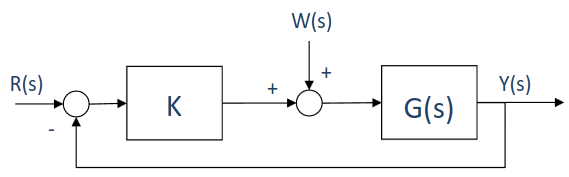
\includegraphics[width = 0.9\linewidth]{img/3/feedback-loop-simp.png}
    \caption{diagrama de blocos simplificado}
    \label{fig:feed-loop-simp}
\end{figure}

\noindent É de fácil observação que a atenuação do efeito de $W$ é mais versátil supondo o modelo em malha fechada:

$$
    Y(s) = \dfrac{KG(S)}{1 + KG(s)}R(s) + \boxed{\dfrac{G(s)}{1 + KG(s)}W(s)}
$$

\noindent A influência de $W(s)$ é atenuada através do incremento de $K$. \textbf{A saída é tanto menos afetada por $W$ quanto maior for o ganho do controlador, $K$}. Assim, é possível enunciar as seguintes observações:

\begin{itemize}
    \item Boa rejeição da perturbação $W$ aumentar $|KG(jw)|$
    \item Bom seguimento da referência r (erro pequeno) aumentar $|KG(jw)|$
\end{itemize}

\noindent Supondo agora um modelo que inclua a adição de uma componente $V$ de ruído (de forma análoga à verificada na \hyperref[fig:feed-loop]{fig. 6}), obtemos a seguinte expressão de saída:

$$
    Y(s) = \dfrac{KG(S)}{1 + KG(s)}R(s) + \boxed{\dfrac{G(s)}{1 + KG(s)}W(s) + \dfrac{KG(S)}{1 + KG(s)}V(s)}
$$

\noindent O ruído, cuja \textbf{mitigação passa pela diminuição de $K$}, apresenta habitualmente componentes espectrais de mais alta frequência do que as do sinal de referência. Assim, tipicamente é realizada a seguinte estratégia de controlo:

\begin{itemize}
    \item A baixas frequências, $|KG(jw)| >> 1$
    \item A altas Frequências (nas quais encontramos a banda do ruído) $|KG(jw)| <<1$
    \item Nas frequências intermédias as condições a impor ao ganho estão relacionadas com a
estabilidade em cadeia fechada (já que a alteração do ganho provoca alterações na localização dos pólos do sistema). 
\end{itemize}

%//==============================--@--==============================//%
    %//==============================--@--==============================//%
\newpage
\subsection[3.3 Root Locus ]{\hspace*{0.075 em}\raisebox{0.2 em}{$\pmb{\drsh}$} Root Locus}

\begin{theo}[\underline{Método Root Locus}]{def:ft}\label{def:root-locus}
    \noindent ``The root locus is a graph of the roots of the characteristic polynomial as a function of a parameter, and the method gives insight into the effects of the controller parameter"\cite{medeiros:FSAISE}
\end{theo}

\noindent O \textit{root locus} garante uma caracterização da variação da localização dos pólos do sistema em função do ganho $K$, é um método gráfico que permite avaliar a localização dos pólos da f.t.c.f. sem fatorizar o polinómio denominador dessa f.t. Supondo a seguinte função de transferência e a respetiva função característica:

$$
    T(s) = \dfrac{KG(s)}{1 + KG(s)H(s)}\qquad
    KG(s)H(s) = -1
$$

\noindent É possível enunciar duas condições essenciais através da equação característica do sistema:

$$
    |KG(s)H(s)| = 1\qquad
    \arg(KG(s)H(s)) = (2k + 1)\pi\;\, k \in \mathbb{Z}
$$

\begin{itemize}
    \item \textbf{Condição de módulo:} A condição de módulo permite calcular o valor de K correspondente a cada localização particular das raízes sobre o lugar geométrico.
    \item \textbf{Condição de argumento:} A condição de argumento permite determinar os pontos do plano que pertencem ao \textit{root locus}.
\end{itemize}

\noindent Com base nestas duas condições, são enunciadas um conjunto de regras para construção do \textit{root locus}

%//==============================--@--==============================//%
\subsubsection[3.3.1 Regra 1 --- Número de ramos]{$\pmb{\rightarrow}$ Regra 1 --- Número de ramos}

\noindent Supondo a seguinte função de transferência em cadeia aberta:

$$
    KG(s)H(s) = K\dfrac{N(s)}{D(s)}
$$

\noindent Assumindo a função de transferência como própria, o número de \textbf{ramos} --- lugar geométrico definido por um pólo do sistema em c.f. quando $K$ varia --- é igual ao número de pólos do sistema em cadeia fechada:

$$
    \boxed{D(s) + KN(s) = 0}
$$
%//==============================--@--==============================//%
\subsubsection[3.3.2 Regra 2 --- Simetria]{$\pmb{\rightarrow}$ Regra 2 --- Simetria}

\noindent Os pólos de sistemas realizáveis (sistemas físicos) são:

\begin{itemize}
    \item Reais.
    \item Complexos, ocorrendo em pares conjugados.
\end{itemize}

\noindent Este último caso indica que o \textit{root locus} é \textbf{simétrico relativamente ao eixo real}.

%//==============================--@--==============================//%
\subsubsection[3.3.3 Regra 3 --- Troços sobre o eixo real]{$\pmb{\rightarrow}$ Regra 3 --- Troços sobre o eixo real}

\noindent Para um ganho, $K$, positivo, são troços do \textit{root locus} os pontos do eixo real que tenham à sua direita um número ímpar de pólos e zeros da f.t.c.a. Neste sentido invocamos a condição de argumento:

$$
    \arg(KG(s)H(s)) = \sum_{i = 1}^{m}\arg(s + z_i) - \sum_{i = 1}^{m}\arg(s + p_i) = (2k + 1)\pi
$$
\noindent Por interpretação direta da expressão acima, reconhecemos que:
\begin{itemize}
    \item Pólos e zeros (f.t.c.a.) à esquerda de s1 contribuem com 0º.
    \item Pólos e zeros (f.t.c.a.) à direita de s1 contribuem com 180º.
    \item A contribuição de um par de pólos e ou de zeros complexos conjugados é nula (``since they contribute no net angle to the real axis").
\end{itemize}

%//==============================--@--==============================//%
\subsubsection[3.3.4 Regra 4 --- Ponto de partida dos ramos]{$\pmb{\rightarrow}$ Regra 4 --- Ponto de partida dos ramos}

\noindent O ponto de partida de cada ramo do \textit{root locus} pressupõe que $K = 0$. Neste sentido, avaliando a expressão já previamente abordada na regra 1:

$$
   \begin{aligned}
       D(s) + KN(s) &= 0,\;\, K \to 0^+\\[4pt]
       \Aboxed{D(s) &= 0}
   \end{aligned}
$$

\noindent Os pontos de partida dos ramos do root-locus coincidem com os pólos da f.t.c.a.

%//==============================--@--==============================//%
\subsubsection[3.3.5 Regra 5 --- Ponto de chegada dos ramos]{$\pmb{\rightarrow}$ Regra 5 --- Ponto de chegada dos ramos}

\noindent O ponto de chegada de cada ramo do \textit{root locus} pressupõe que $K \to \infty$. Fazendo uso da condição de magnitude:

{
\mdfsetup{linewidth=2pt}

\begin{mdframed}
    \noindent Quando $K \to \infty$ é necessário que $G(s)H(s) \to 0$ para que $1 + KG(s)H(s) = 0$
\end{mdframed}
}

\noindent Verificam-se assim duas situações:
\begin{itemize}
    \item $s \to \{\text{zeros de } N(s)\}$ --- m ramos tendem para os zeros da f.t.c.a.
    \item $s \to \infty$ --- n-m ramos tendem para $\infty$, se o denominador possuir mais pólos que zeros.
\end{itemize}

%//==============================--@--==============================//%
\subsubsection[3.3.6 Regra 6 --- Pontos de entrada e de saída do eixo real]{$\pmb{\rightarrow}$ Regra 6 --- Pontos de entrada e de saída do eixo real}

\noindent Para encontrar o ponto onde o \textit{root locus} se afasta do eixo real (ou converge para o eixo real), observamos que tal ocorre sempre que duas (ou mais) raízes se intersectam.  É um facto bem conhecido que, quando um polinómio tem várias raízes, não só o valor do polinómio é zero, como a sua derivada também o é.

\vspace{1 em}
\noindent Nos pontos de saída (e de entrada), a derivada da equação característica é zero, onde:
\begin{itemize}
    \item O ponto de saída do eixo real ocorre para um máximo relativo do ganho.
    \item O ponto de entrada no eixo real ocorre para um mínimo relativo do ganho
\end{itemize}

$$
    \begin{aligned}
        \dfrac{d}{ds}\left(1 + K\dfrac{N(s)}{D(s)}\right) = 0\qquad
        &K \left(\dfrac{N(s)'D(s) - N(s)D(s)'}{D(s)^2}\right) = 0\\[6pt]
        \Aboxed{N(s)'D(s) &- N(s)D(s)' = 0}
    \end{aligned}
$$

\noindent\textbf{Nota:} Nem todas as soluções desta equação são sempre pontos de saída ou de entrada no eixo real, é preciso confirmar se as soluções encontradas estão sobre troços que pertencem ao \textit{root locus}

%//==============================--@--==============================//%
\subsubsection[3.3.7 Regra 7 --- Ângulos de partida e de chegada ao eixo real]{$\pmb{\rightarrow}$ Regra 7 --- Ângulos de partida e de chegada ao eixo real}

\noindent De forma sucinta, O ângulo entre dois ramos adjacentes que se aproximam (ou que se afastam) do mesmo ponto do eixo real é dado por:

$$
    \boxed{\sigma = \dfrac{2\pi}{\alpha}}
$$

\noindent O ângulo entre dois ramos adjacentes, um chegando e outro partindo do mesmo ponto do eixo real é dado por:

$$
    \boxed{\sigma = \dfrac{\pi}{\alpha}}
$$

\noindent Onde $\alpha$ é o número de ramos que se cruzam num ponto do eixo real.
%//==============================--@--==============================//%
\subsubsection[3.3.8 Regra 8 --- Comportamento Assintótico]{$\pmb{\rightarrow}$ Regra 8 --- Comportamento Assintótico}

\noindent Quando $K \to \infty$ existem $n - m$ ramos que tendem para infinito ao longo de assíntotas. Estas assíntotas cruzam-se no ponto do eixo real (centro assíntótico) segundo:

$$
    \boxed{\dfrac{\sum \text{pólos de }G(s)H(s) - \sum \text{zeros de }G(s)H(s)}{n - m}}
$$

\noindent O ângulo de partida com o eixo real é dado por:
$$
    \boxed{\Phi_a = \dfrac{\pm (2k + 1)\pi}{n - m},\;\, k = 0,1,2,\dots n-m-1}
$$
%//==============================--@--==============================//%
\subsubsection[3.3.9 Regra 9 --- Soma dos pólos]{$\pmb{\rightarrow}$ Regra 9 --- Soma dos pólos}

\noindent Supondo a seguinte  f.t.c.a:

$$
    G(s)H(s) = \dfrac{N(s)}{D(s)}
$$

\noindent Se $n - m \ge 2$ então:

$$
    \boxed{\sum \text{pólos da f.t.c.a} = \sum \text{pólos da f.t.c.f.}}
$$

\noindent\textbf{Nota:} Esta propriedade tem particular interesse para deduzir pólos da f.t.c.f e vice-versa.
%//==============================--@--==============================//%
    %//==============================--@--==============================//%
\newpage
\subsection[3.4 Controlador PID]{\hspace*{0.075 em}\raisebox{0.2 em}{$\pmb{\drsh}$} Controlador PID}

\noindent ``Starting with simple proportional feedback, engineers early discovered integral control action as a means of eliminating bias offset. Then, finding poor dynamic response in many cases, an “anticipatory” term based on the derivative was added. The result is called the three-term or PID controller, and has the transfer function"\cite{FranklinPowell2015}

$$
    \boxed{D_c(s) = K_p + \dfrac{K_i}{s} + s \cdot K_d}
$$

\noindent Este controlador possui três ações ajustáveis --- Proporcional (\textbf{p}), Integral (\textbf{i}), Derivativa (\textbf{d}) --- com o objetivo de  melhorar a seguimento da referência e/ou rejeitar as perturbações e melhorar a resposta transitória.

%//==============================--@--==============================//%
\subsubsection[3.4.1 Ação proporcional]{$\pmb{\rightarrow}$ Ação proporcional}
\noindent Quando o sinal de controlo de realimentação é linearmente proporcional ao erro do sistema:
$$
    u(t) = K_p e(t)
$$

\noindent Designamos o resultado por retroação proporcional. Assim, o sinal de controlo varia linearmente com o erro do sistema. Se $K_p$ for grande o suficiente para obter um erro em regime estacionário adequadamente pequeno, \textbf{o amortecimento tornar-se-á demasiado pequeno} para a obtenção de uma resposta transitória satisfatória (apenas com controlo proporcional)

\begin{figure}[H]
    \centering
    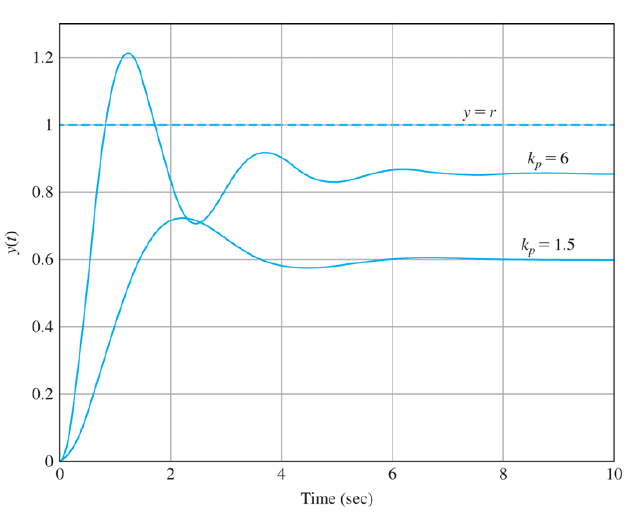
\includegraphics[width = 0.5\linewidth]{img/3/proportional-control.png}
    \caption{Efeito da ação proporcional para vários valores de $K_p$.}
    \label{fig:proportional-control}
\end{figure}

%//==============================--@--==============================//%
\subsubsection[3.4.2 Ação integral]{$\pmb{\rightarrow}$ Ação integral}
\noindent Quando um sinal de controlo de realimentação é linearmente proporcional ao integral do erro do sistema, chamamos ao resultado \textbf{realimentação integral}. 
$$
    u(t) = K_i \int e(\tau)\, d\tau
$$

\noindent $K_i$ designa-se ganho integral. A ação integral garante que, o sinal de controlo, em cada instante de tempo é um somatório de todos os valores passados do erro de seguimento.

\begin{figure}[H]
    \centering
    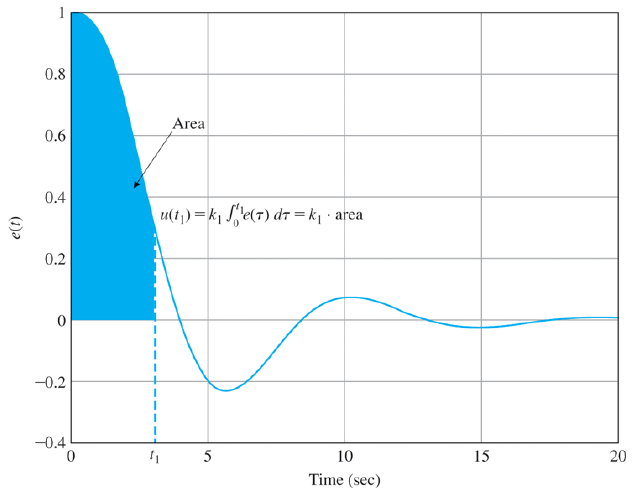
\includegraphics[width = 0.5\linewidth]{img/3/integral-control.png}
    \caption{``Integral control is based on the history of the system error"\cite{FranklinPowell2015}.}
    \label{fig:integral-control}
\end{figure}

\noindent A ação integral tem a principal virtude de poder fornecer um valor finito de controlo com erro de seguimento nulo. Tal acontece porque $u(t)$ é uma função de todos os valores passados de $e(t)$ e não apenas do valor no instante atual. Admitindo que o sistema da \hyperref[fig:feed-loop]{fig.6} possui um controlador integral, obtemos:

$$
    \dfrac{E(s)}{R(s)} = \dfrac{s}{s + K_i G(s)}\qquad
    \dfrac{Y(s)}{R(s)} = \dfrac{K_i G(s)}{s + K_i G(s)}\qquad
    \dfrac{U(s)}{R(s)} = \dfrac{K_i}{s + K_i G(s)}
$$

\noindent Assumindo como entrada o degrau unitário e aplicando o teorema do valor final:

$$
    e(\infty) = 0\quad
    y(\infty) = 1\quad
    u(\infty) = 1
$$
\noindent Note-se que o erro de seguimento em regime estacionário será zero, qualquer que seja o valor de $K_i$. O ganho integral $K_i$ é meramente selecionado para proporcionar uma resposta dinâmica aceitável. aceitável; no entanto, O seu incremento excessivo poderá causar instabilidade. Neste sentido podemos afirmar o seguinte:

\begin{itemize}
    \item melhor seguimento em regime permanente.
    \item pior estabilidade relativa --- os pólos infletem para o s.p.c.d com o aumento de $K_i$.
\end{itemize}

\noindent Consequentemente é relevante falar do \textbf{controlador integral proporcional}:
$$
    K_p \cdot \left[1 + \dfrac{1}{T_s s}\right] = K_p \cdot \dfrac{s + 1/T_s}{s}
$$

\begin{itemize}
    \item melhor seguimento em regime permanente.
    \item zero em $s = -1/T_s$, normalmente colocado perto do pólo referente ao integrador de modo a não destabilizar a dinâmica do sistema.
    \item \textbf{melhora o seguimento em regime permanente}, sem alterar significativamente os ramos principais do root-locus.
\end{itemize}
%//==============================--@--==============================//%
\newpage
\subsubsection[3.4.3 Ação derivativa]{$\pmb{\rightarrow}$ Ação derivativa}
\noindent O objetivo da ação derivativa é melhorar a estabilidade do sistema em malha fechada, bem como acelerar a resposta transitória e reduzir o \textit{overshoot}.

$$
    u(t) = K_d \Dot{e}(t)
$$

\noindent A ação derivativa quase nunca é utilizado por si só, é assim relevante referir o \textbf{controlador porporcional derivativo} e o \textbf{controlador proporcional integral derivativo}, respetivamente:

\vspace{1em}
\noindent \textbf{Controlador porporcional derivativo}
$$
    K_pT_d\cdot(s + 1/T_d)
$$
\begin{itemize}
    \item “atrai” os ramos do root-locus afastando-os do s.p.c.d --- aumenta $\gamma$ (amortecimento)
    \item introduz “antecipação” --- $u(t)$ depende não só da intensidade do erro $e(t)$ (\textbf{ação P}), mas também da sua rapidez de variação (\textbf{ação D}).
    \item amplifica as componentes de alta frequência dos sinais.
\end{itemize}

\noindent \textbf{Controlador proporcional integral derivativo}
$$
    K_pT_d\cdot(s + 1/T_d)\cdot \dfrac{(s + 1/T_i)}{s}
$$
\begin{itemize}
    \item Reúne as ações anteriores.
    \item Partindo do controlador PD, introduz-se um polo na origem e um zero perto da origem.
    \item A substituição PD por PID melhora o seguimento em regime permanente, sem alterar significativamente os ramos principais do root-locus.
\end{itemize}

{
\mdfsetup{linewidth=2pt}

\begin{mdframed}
    \noindent O desenho de um controlador envolve sempre a implementação inicial de um controlador Proporcional-Derivativo (\textbf{PD}), que é responsável pelas características transitórias do sistema. Tal é seguido pela implementação de um controlador Proporcional-Integral (\textbf{PI}) para eliminar o erro em regime estacionário.
\end{mdframed}
}

    \clearpage
    \section{Resposta em frequência}
    %//==============================--@--==============================//%
\subsection[4.1 Diagrama de Bode e Relação Tempo-Frequência]{\hspace*{0.075 em}\raisebox{0.2 em}{$\pmb{\drsh}$} Diagrama de Bode e Relação Tempo-Frequência}
``The most useful technique for hand plotting was developed by H. W. Bode at Bell Laboratories between 1932 and 1942. The idea in Bode's method is to plot magnitude curves using a logarithmic scale and phase curves using a linear scale. This strategy allows us to plot a high-order $G(j\omega)$ by simply adding the separate terms graphically.
$$
    \frac{\bar{s}_1 \bar{s}_2}{\bar{s}_3 \bar{s}_4 \bar{s}_5} = \frac{r_1 e^{j\theta_1} r_2 e^{j\theta_2}}{r_3 e^{j\theta_3} r_4 e^{j\theta_4} r_5 e^{j\theta_5}} =
    \left( \frac{r_1 r_2}{r_3 r_4 r_5} \right) e^{j(\theta_1 + \theta_2 - \theta_3 - \theta_4 - \theta_5)}
$$
phases of the individual terms are added directly to obtain the phase of the composite expression, $G(j\omega)$. Furthermore, because
$$
    \vert G(j\omega) \vert = \frac{r_1 r_2}{r_3 r_4 r_5}
$$
it follows that
$$
    \log_{10}\vert G(j\omega) \vert = \log_{10}(r_1) + \log_{10}(r_2) - \log_{10}(r_3) - \log_{10}(r_4) - \log_{10}(r_5).\text{''\cite{FranklinPowell2015}}
$$

\begin{figure}[H]
    \centering
    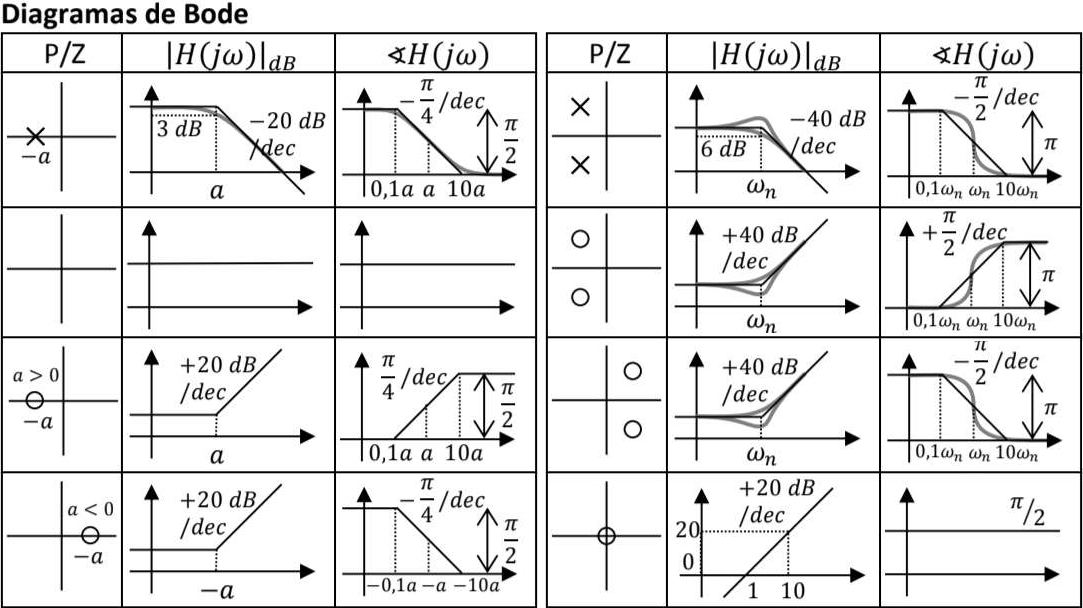
\includegraphics[width = 0.7\linewidth]{img/3/bode.png}
    \caption{Resposta assimtótica---resposta em diagramas de Bode.}
    \label{fig:bode}
\end{figure}

\noindent\textbf{Largura de banda} --- Banda de frequência na qual o módulo da função resposta em frequência não cai mais de 3dB em relação ao ganho de baixa frequência, traduz a capacidade de um sistema reproduzir mais ou menos perfeitamente os sinais aplicados à sua entrada.
%//==============================--@--==============================//%
\subsection[4.2 Critério de Nyquist]{\hspace*{0.075 em}\raisebox{0.2 em}{$\pmb{\drsh}$} Critério de Nyquist}

\noindent``The Nyquist stability criterion relates the open-loop frequency response to the number of closed-loop poles of the system in the RHP."\cite{FranklinPowell2015}

\vspace{1em}
\begin{itemize}
    \item Calcula a estabilidade do sistema em cadeia fechada sem avaliar explicitamente os pólos da f.t.c.f.
    \item Dá indicações sobre estabilidade relativa, através das margens de ganho e de fase.
\end{itemize}

\noindent Usa resultados da teoria das funções complexas (Teorema de Cauchy) para estudar a existência de zeros de $1+KG(s)H(s)$ no semi-plano complexo direito ou sobre o eixo imaginário.

%//==============================--@--==============================//%
\subsubsection[4.2.1 Teorema de Cauchy (Princípio do argumento)]{$\pmb{\rightarrow}$ Teorema de Cauchy (Princípio do argumento)}

{
\mdfsetup{linewidth=2pt}

\begin{mdframed}

    \begin{enumerate}
    \item Let $Z$ and $P$ be the number of zeros and poles of $L(s)$ inside $\Gamma$.
    \item As $s$ moves around $\Gamma$, $\angle L(s)$ undergoes a net change of $-(Z - P)2\pi$.
    \item A net change of $-2\pi$ means that the vector from $0$ to $L(s)$ swings clockwise around the origin one full rotation.
    \item A net change of $-(Z - P)2\pi$ means that the vector from $0$ to $L(s)$ must encircle the origin in a clockwise direction $(Z - P)$ times.
    \end{enumerate}

    \begin{theo}[\underline{Cauchy's Principle of the Argument}]{teo:cauchy}\label{teo:cauchy}
    Consider a transfer function $L(s)$ and a simple closed clockwise contour $\Gamma$. Let $Z$ and $P$ be the number of zeros and poles of $L(s)$ inside $\Gamma$.
    \begin{itemize}
    \item Then, the contour generated by evaluating $L(s)$ along $\Gamma$ will encircle the origin in a clockwise direction $Z - P$ times.
    \end{itemize}
    \end{theo}

    \begin{figure}[H]
        \centering
        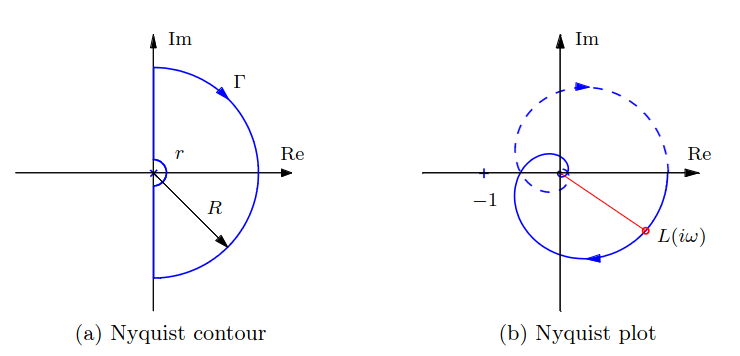
\includegraphics[width = 0.8\linewidth]{img/4/cauchy-arg-theorem.png}
        \label{fig:cauchy-theorem}
    \end{figure}
\end{mdframed}
}

A estabilidade em cadeia fechada é obtida se:
\begin{itemize}
    \item $N = 0$
    \item $Z = -P$
\end{itemize}

\noindent Assim, um sistema causal com f.t.c.a $KG(s)$ é estável em cadeia fechada sse

\begin{theo}[\underline{Critério de Nyquist}]{teo:Nyq}\label{teo:Nyq}
    Quando o afixo de s percorre o contorno de Nyquist num determinado sentido, o número de voltas que o afixo de $KG(s)$ percorre em torno do ponto –1 em sentido contrário é igual ao número de pólos da $KG(s)$ no interior do contorno de Nyquist.
\end{theo}

%//==============================--@--==============================//%

    %% appendix
    %\appendix
    %

    %% refs
    \clearpage
    \bibliographystyle{unsrtnat}
    \nocite{*}
    {\footnotesize%
    \bibliography{refs}}
    %% attachments
    %\newpage
    %\input{appendix}

\end{document}%